\documentclass[resume]{subfiles}


\begin{document}
\section{Mémoires}
\begin{itemize}
\item RAM
\item ROM
\item CAM
\item FIFO
\end{itemize}
Amélioration dans le Spartan-6 : LUT4 $\rightarrow$ LUT6 pour de meilleures performances.\\
Les BRAM sont disposées à côté des CLB pour améliorer la vitesse.
\begin{itemize}
\item SliceX (\SI{50}{\percent}) : LUT6, 8 flip-flop
\item SliceL (\SI{25}{\percent}) : + MUX, Carry
\item SliceM (\SI{25}{\percent}) : + distributed RAM, shift register
\end{itemize}
\begin{figure}[H]
\centering
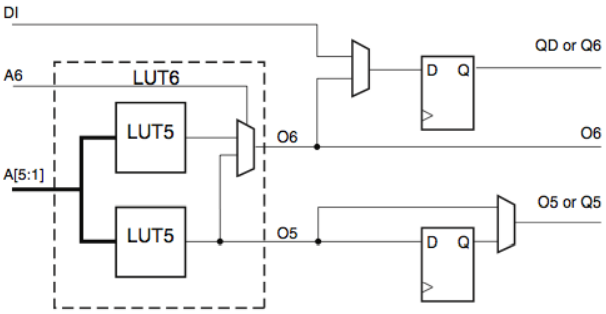
\includegraphics[width=\columnwidth]{img_0.png}
\end{figure}
\subsection{Mémoire on-chip vs externe}
\begin{itemize}
\item On-chip
\begin{itemize}
\item Machines d'état
\item FIFO
\item Stockage local et/ou important
\item \textbf{Rapidité}
\end{itemize}
\item Externe
\begin{itemize}
\item Memory Controller Block (MCB)
\item Flexible
\item Très grande capacité
\item 
\end{itemize}
\end{itemize}








\end{document}